\chapter{The Research Work} 
In this part, we'll see how the theoretical knowledge in Argumentation Theory and NLP presented were applied to a concrete case study. We'll first see the types of textual data we have, how they were annotated for the supervised learning task and then how features were engineered to perform an automatic classification.
\section{Text Corpus}
The data set used for this study was originally composed of 990 text files. They contain forum posts or articles about 6 different domains related to education, that provoke debate in the American society:
\begin{itemize}
  \item \textbf{homeschooling}: It's the education of children outside the formal settings of public or private schools and is usually undertaken directly by parents or tutors. 
  \item \textbf{redshirting}: The practice of postponing entrance into kindergarten of age-eligible children in order to allow extra time for socioemotional, intellectual, or physical growth. 
  \item \textbf{prayer in schools}: Debate about whether or not a public school should allow and allocate time and buildings for religious practices.
  \item \textbf{public vs private schools}: Which kind of school offers the best education.
  \item \textbf{mainstreaming}: In the context of education, it's the practice of educating students with special needs in regular classes during specific time periods based on their skills.
  \item \textbf{single sex education}: The practice of conducting education where male and female students attend separate classes or in separate buildings or schools.  
\end{itemize} 

The meta-information for each text (id, type of post, domain) is given my the name of the file in itself such as follow:

\centerline{\texttt{174\_P2\_artcomment\_homeschooling.txt}}

$\frac{ \textrm{Text}}{1} \frac{\textrm{Text}}{2} \frac{\textrm{Text}}{3}$
??FIND A WAY TO DO IT THIS WAY 

Later in the internship, I started to use \textit{XMI} files\footnote{The XML Metadata Interchange (XMI) is an Object Management Group (OMG) standard for exchanging metadata information via Extensible Markup Language (XML).} that contain more information about the post or comment in itself such as the author, the date, ect... ??Annexe with how xmi looks like ?

\subsection{Manual Annotation}
As mentioned before, the classification we want to perform is a supervised learning problem since it wants to imitate the human decision on judging if a post is persuasive or not. An annotation guideline was written by Ivan Habernal \cite{ivanguideline} in order for the annotators to understand the task. In this section, we'll discuss about the general ideas of this guideline.
\subsubsection{Sources of the data}
The textual data that will be used for the studies come from to kind of online sources:
\\
\texttt{artcomment: Article Comments, reactions to online articles}
\\
\texttt{forumpost: Forum Posts, posts in online debates}
\subsubsection{Categories in Persuasion}
\textbf{The task}: Distinguish, whether the comment is persuasive regarding the discussed topic. The key question to answer is: \textit{Does the author intend to convince us clearly about his/her attitude or opinion towards the topic?} If the answer is yes, we classify the comment as persuasive. There are two main categories in this task, namely \texttt{P1:Persuasive} and \texttt{P2:Non-persuasive}. The second category is further divided into more categories, that basically cover the various phenomena that may be encountered in the data.

However, It is not necessary to categorize the data exactly into one of the categories under \texttt{P2:Non-persuasive}. For example, a particular text may be both off-topic and out-of-context; in that case, choose either of these categories.
\\
Remember: we are mainly interested in finding the \texttt{P1:Persuasive} documents that represent on-topic texts with intentions to persuade and convince the readers.
\vspace{0.1cm}
\\
\texttt{Quick overview of possible distinct categories:}
\\
\texttt{P1: Persuasive}
\\
\texttt{P2: Non-persuasive}

\texttt{P2.1: Out-of-context or reaction to other comment}

\texttt{P2.3: Off-topic}

\texttt{P2.4: Personal worries}

\texttt{P2.5: Story-sharing without intentions to persuade}

\texttt{P2.7: Impossible to decide about persuasiveness without deep background knowledge}
\\
\vspace{0.15cm}
While the annotation phase, the annotators were charged of determining if a text was in the P1 class and if not they had to specify to which of the seven P2 subclasses it belongs to.

\subsubsection{Examples}
\textbf{Clearly belongs to P1}
\\
\\
\fbox{\begin{minipage}{1\textwidth}
\textbf{\#2013 (forumpost, single-sex-education)} School should be co-ed. Some children are
awkward with others of their own gender. For example, certain girls who are tom-boys might not be comfortable in a room full of girls. The mixed genders are preparing kids for the real world, where things are not segregated.
\end{minipage}}
\\
\\
In \texttt{\#2013}, the author states that schools should not be single-sex, also provides reasons why he/she thinks so.
\\
\\
\textbf{Problematic P1 case}
\\
\\
This section discusses some examples that were marked as P1 by two annotators but as P2 by a third annotator. We will explain, where the third annotator made an error.
\\
\\
\fbox{\begin{minipage}{1\textwidth}
\textbf{\#300 (artcomment, homeschooling)} This is not representative of most homeschoolers. This is a very, very small minority. Let’s compare that to entire schools in the public school system that cater their teaching to make sure their kids pass the standardized tests so they can keep funding, meanwhile the kids can’t understand concepts that aren’t covered on the tests.

I was homeschooled in Texas, where there is no government oversight of homeschooling. I graduated high school at age 16 with 24 college credits under my belt, was accepted into every university I applied to (all the major schools in Texas), and graduated college in three years at age 19 after being on the Dean’s List every semester except one. Neither of my parents has a college degree and would not be deemed ``qualified'' to teach me. Somehow I didn’t just make it, I thrived. Parental involvement works.
\end{minipage}}
\\
\\
The second paragraph in \texttt{\#300} contains a statement ``parental involvement works'', which is clearly in favor of homeschooling.
\\
\\
\textbf{P2.1: Non-persuasive, out-of-context or reaction to other comment}
\\
\\
\fbox{\begin{minipage}{1\textwidth}
\textbf{\#3245 (artcomment, public-private-schools)} Why are they bad, they still pay taxes but don’t use the service so there is more money for the system to use on fixing its issues. Even when everyone is doing everything they can to fix something does not mean it will be fixed.
\end{minipage}}
\\
\\
In \texttt{\#3245}, without any context, we can only roughly guess what the author is writing about.
\\
\\
\textbf{P2.3: Non-persuasive, off-topic}
\\
\\
\fbox{\begin{minipage}{1\textwidth}
\textbf{\#2049 (artcomment, single-sex-education)} Single-sex education. A poem./ Dearest
people, the people/ always arguing and full of hate,/ why oh why should we ever/ turn out this way? Single-sex,/ co-educational, why does it matter?/ Girls, boys, everyone;/ WE CANNOT REMAIN LIKE THIS/ do you hear me?
\end{minipage}}
\\
\\
\textbf{P2.4: Non-persuasive, personal worries}
\\
\\
\fbox{\begin{minipage}{1\textwidth}
\textbf{\#5024 (artcomment, redshirting)} Oh boy. . . oh my little (but very tall) girl. I’ve chosen to put her into a second year of preschool next year (5 days instead of 3) because I feel that's what is right for her. She's a late October baby, but I'm not sure she's ready for kindergarten. But I worry. Will she be the giant of her class every year? Will there be an opportunity to skip her a grade? She's quite bright, but socially still a little awkward. I don't feel I'm ``holding her back", yet if she has brand new twin sisters arriving in July, should I totally turn her world upside down and ship her off to another school with mostly older kids? I'm torn (and totally on the fence) both ways. I want her to excel academically, but I don't want to throw too many changes at her at once. I'm with you, Erica. I'm torn, and I chose the now unpopular ``redshirting", but not so she can be a hockey superstar. . . :) I just thought this was a better pace for her. In ten years, I'm sure the ``experts" will be telling me I should have held
her back, because all the young kids are struggling. . . You can't win.
\end{minipage}}
\\
\\
In \texttt{\#5024}, the author only expresses her worries about her child, but she neither takes stance on the topic nor argues about that.
\\
\\
\textbf{P2.5: Non-persuasive, story-sharing without intentions to persuade}
\\
\\
\fbox{\begin{minipage}{1\textwidth}
\textbf{\#5030 (artcomment, redshirting)} Born in November, my youngest sister was among the oldest children in her peer group until she skipped a grade (I believe she skipped grade one but it may have been grade two). My other sister, also born in November and two years older, showed my youngest sister her homework and my youngest sister proved such a quick learner the teacher had no choice but to recommend she be moved up. She’s still achieving plenty and has never been intimidated by anyone older. She has a competitive drive and enjoys pushing herself forward.
\end{minipage}}
\\
\\
The purpose of \texttt{\#5030} was to share the story without taking stance towards the topic or persuading others (the story of her sister skipping a grade and doing well could is also too far from the redshirting topic).
\\
\\
\textbf{P2.7: Non-persuasive, impossible to decide about persuasiveness without deep back-ground knowledge}
\\
\\
\fbox{\begin{minipage}{1\textwidth}
\textbf{\#164 (artcomment, homeschooling)}: Child abuse in the name of religious freedom. Just like parents who refuse medical treatment for their children. It makes me wish there was a hell.
\end{minipage}}
\\
\\
In \texttt{\#164}, without knowing the context that homeschooling and religion education are somehow related issues in some communities, it is not possible to decide about persuasiveness of this document.

\subsubsection{Annotation Process}
Three annotators were charged of labelling the data as P1 and P2 (if P2, he was asked to specify the subclass). For every annotations, the annotator could write a comment about why he thinks the text can be considered as persuasive or not. This comment can be useful especially if there's a conflict among the 3 annotators. 

Once the annotations are performed, a discussion takes place with the annotators in order to solve issues and conflict annotations. If all annotators agree on the class (P1 or P2) of a text, the class will be set as the \emph{gold label} of this text. But if after the discussion, there's still a conflict, the text will be labelled according to majority. 

To evaluate how well were the annotations, we compare statistical metrics that are described in~\cref{sec:stanabin} such as Recall, Precision, Accuracy and Macro $F_{1}$ measure. The comparison will be performed on 4 scenario: 
\begin{itemize}
  \item \textbf{$A_1$ vs $A_2$}
  \item \textbf{$A_1$ vs $A_3$}
  \item \textbf{$A_2$ vs $A_3$}
  \item 3 Annotators \textbf{vs} \Gls{gold data}
\end{itemize}
$A_1$, $A_2$, $A_3$ stand for Annotator number 1, 2 and 3. 

\subsubsection{Results of the Manual Annotations}
We measure the performances of the annotations on 3 batches of text data, and we aggregate the results:
\begin{table}[H]
\begin{tabular}{lrrr|rrr|rrr}
	&	&	&	& \multicolumn{3}{l}{Persuasive} & \multicolumn{3}{l}{Non-Persuasive} \\
	& Docs	& Macro $F_1$ & Acc. & P & R	& $F_1$ & P & R & $F_1$ \\ \hline
Batch 1	&	&	&	&	&	&	&	&	&\\
A1	&100	&0.879	&0.880	&0.942	&0.845	&0.891	&0.813	&0.929	&0.867\\
A2	&100	&0.895	&0.900	&0.875	&0.966	&0.918	&0.944	&0.810	&0.872\\
A3	&100	&0.849	&0.850	&0.922	&0.810	&0.862	&0.776	&0.905	&0.835\\ \hline
Batch 2	&	&	&	&	&	&	&	&	&\\
A1	&200	&0.855	&0.855	&0.909	&0.792	&0.847	&0.813	&0.919	&0.863\\
A2	&200	&0.910	&0.910	&0.919	&0.901	&0.910	&0.901	&0.919	&0.910\\
A3	&200	&0.874	&0.875	&0.839	&0.931	&0.883	&0.920	&0.818	&0.866\\ \hline
Batch 3	&	&	&	&	&	&	&	&	&\\
A1	&509	&0.927	&0.927	&0.953	&0.906	&0.929	&0.902	&0.950	&0.926\\
A2	&502	&0.879	&0.884	&0.836	&0.986	&0.905	&0.977	&0.757	&0.853\\
A3	&511	&0.907	&0.908	&0.977	&0.835	&0.900	&0.857	&0.981	&0.915\\ \hline
All data	&	&	&	&	&	&	&	&	&\\
A1	&809	&0.904	&0.904	&0.942	&0.871	&0.905	&0.867	&0.940	&0.902\\
A2	&802	&0.890	&0.893	&0.858	&0.964	&0.908	&0.948	&0.807	&0.872\\
A3	&811	&0.893	&0.893	&0.929	&0.855	&0.890	&0.861	&0.932	&0.895\\
\end{tabular}
\caption{\label{tab:human-performance-annotation-study-1} Human performance on \emph{gold data persuasive}.}
\end{table}
??help: Find a way to say the results are good that's why we want to do a text classification.

\subsection{Corpus Statistics}
Now that we have the \emph{gold labels} for the texts, we can sum the relevant information in a table: 
\begin{table}[h]
\begin{tabular}{ll|l|l|l|l|l|l|l|}
\cline{3-9}
 &  & redshirting & prayer-in-schools & homeschooling & single-sex-education & mainstreaming & public-private-schools & Total \\ \hline
\multicolumn{1}{|l|}{} & artcomment & 24 & 60 & 64 & 17 & 1 & 278 & 444 \\ \cline{2-9} 
\multicolumn{1}{|l|}{} & forumpost & 14 & 17 & 22 & 9 & 9 & 9 & 80 \\ \cline{2-9} 
\multicolumn{1}{|l|}{\multirow{-3}{*}{P1}} & \cellcolor[HTML]{C0C0C0}all & \cellcolor[HTML]{C0C0C0}38 & \cellcolor[HTML]{C0C0C0}77 & \cellcolor[HTML]{C0C0C0}86 & \cellcolor[HTML]{C0C0C0}26 & \cellcolor[HTML]{C0C0C0}10 & \cellcolor[HTML]{C0C0C0}287 & \cellcolor[HTML]{C0C0C0}524 \\ \hline
\multicolumn{1}{|l|}{} & artcomment & 15 & 43 & 93 & 16 & 2 & 174 & 343 \\ \cline{2-9} 
\multicolumn{1}{|l|}{} & forumpost & 15 & 23 & 45 & 8 & 17 & 15 & 123 \\ \cline{2-9} 
\multicolumn{1}{|l|}{\multirow{-3}{*}{P2}} & \cellcolor[HTML]{C0C0C0}all & \cellcolor[HTML]{C0C0C0}30 & \cellcolor[HTML]{C0C0C0}66 & \cellcolor[HTML]{C0C0C0}138 & \cellcolor[HTML]{C0C0C0}24 & \cellcolor[HTML]{C0C0C0}19 & \cellcolor[HTML]{C0C0C0}189 & \cellcolor[HTML]{C0C0C0}466 \\ \hline
\multicolumn{1}{|l|}{} & Total & 68 & 143 & 224 & 50 & 29 & 476 & 990 \\ \cline{2-9} 
\multicolumn{1}{|l|}{\multirow{-2}{*}{P1  + P2}} & Percentage & 6.9 & 14.4 & 22.6 & 5.1 & 2.9 & 48.1 & 100 \\ \hline
\end{tabular}
\end{table}
??Find a ways for the color and the size

\subsection{Conflict Annotations}
??Mention the conflict annotations + some statistics 
\section{Feature Engineering}
Now that we have all our data annotated, we have to extract relevant information from it in order to perform the classification. The problem of identifying persuasion in a text is a relatively new question in NLP and we don't have any straightforward methodology to find relevant features. Thus, we'll implement the NLP standard features that are used widely in other sub-fields of language processing and then we'll use the state-of-the-art features discovered in Argumentation Mining. A lot of modules of DKPro helped us to create our features but we had to extend somehow the software for certain functionalities that were not in DKPro Core and TC (for example the \emph{Sentiment Analysis}).

\subsection{Lexical Features}   
The adjective lexical refers to the words and the vocabulary of a corpus. This part will deal with the extraction of meaningful features related to words, sentences, \glspl{token}\footnote{Tokenization is the process of breaking a stream of text up into words, phrases, symbols, or other meaningful elements called tokens.}, punctuations, ect...

\subsubsection{Tokens N-Grams}
In NLP, an n-gram is a contiguous sequence of n (with n integer) items from a given sequence of text or speech. As a result of, tokens n-grams are sequences of tokens from a text (\textit{Note: } For more information about units in linguistics such as words, tokens, \gls{lemma} and \gls{stemma}, have a look at~\cref{sec:linmorph}). The study of n-grams distribution in a corpus is an ancient technique \cite{tcjullmann77} in language processing and it's usage is common in the field.

In this study, we use a DKPro available feature that extracts the 10.000 most common 1,2 and 3-grams in all the corpus and returns for each text a 10000-dimensional binary vector. Each vector element corresponds to one of the 10000 extracted n-gram, its value is 1 the text contains the n-grams, 0 otherwise.
\\
To better understand this feature, let's take a simple example. We consider that the set of 1-grams contains 10 elements such as follow: 

\begin{equation*}
E = \{2, 1990, a, born, dog, Frankfurt, in, I, was, zoo\}
\end{equation*}
\\

If the text input is:
\\
\centerline{\texttt{I was born in 1990}}
\\

DKPro will return the following binary 10-dimensional vector:
\begin{table}[h]
\center
\begin{tabular}{llllllllll}
2                       & 1990                   & a                      & born                   & dog                    & Frankfurt              & in                     & I                      & was                    & zoo                    \\ \hline
\multicolumn{1}{|l|}{0} & \multicolumn{1}{l|}{1} & \multicolumn{1}{l|}{0} & \multicolumn{1}{l|}{1} & \multicolumn{1}{l|}{0} & \multicolumn{1}{l|}{0} & \multicolumn{1}{l|}{1} & \multicolumn{1}{l|}{1} & \multicolumn{1}{l|}{1} & \multicolumn{1}{l|}{0} \\ \hline
\end{tabular}
\end{table}

As mentioned before, this feature is already implemented in DKPro and it's easy to use it in a pipeline.
\
\begin{figure}[h]
    \centering
    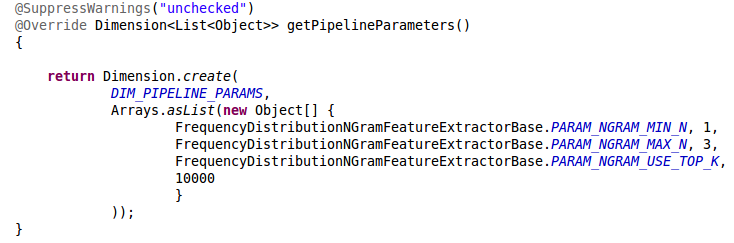
\includegraphics[width=1.05\textwidth]{fig/ngramfeature.png}
    \caption[Short caption]{NGram Feature in DKPro Java code}
    \label{fig:ngramfeature}
\end{figure}
\

As displayed on \ref{fig:ngramfeature}, the n-gram feature extractor takes three parameters: \emph{PARAM\_NGRAM\_MIN\_N} for the minimal value of n, \emph{PARAM\_NGRAM\_MAX\_N} for the maximal value of n and \emph{PARAM\_NGRAM\_USE\_TOP\_K} which is the number of common n-grams retained.
Since we want the 10.000 most common 1,2 and 3-grams, the parameters are set such as follow:

\begin{itemize}[label={}]
  \item \texttt{PARAM\_NGRAM\_MIN\_N = 1}
  \item \texttt{PARAM\_NGRAM\_MAX\_N = 3}
  \item \texttt{PARAM\_NGRAM\_USE\_TOP\_K = 10000}
\end{itemize}

We also implemented a subclass from the n-grams extractors to have the lemma instead of the tokens. We thought that it would give us better results since lemma refer to a general form of a word (ex: \emph{be} instead of \emph{are}, \emph{was}, \emph{is}, ect...) but in \emph{a posteriori} analyses, we don't see any improvements in our results. At the result of, we'll only consider tokens n-grams in our features.

The Tokens N-Grams feature will give us results for our \emph{Baseline Analysis}: more complex models and pipelines will systematically be compared to this ``simple" model.

\subsubsection{Tokens and Sentences}
We compute some statistics regarding sentences and sentences in a text:
\begin{itemize}
  \item Number of sentences and tokens in a text.
  \item Maximum size (in character) of a token and a sentence in a text.
  \item Minimum size (in character) of a token and a sentence in a text.
  \item Average size (in character) of tokens and sentences in a text. 
\end{itemize} 
\
As an example, if we consider the following text as input:
\\
\\
\fbox{\begin{minipage}{1\textwidth}
\textbf{208\_P2\_artcomment\_homeschooling.txt} ``Not having read any of the standard high school literature, people make references I don’t get." 
Got news for you. They're not making references to required high school readings. More likely Internet and pop culture. 
I hope you succeed getting some accountability in to the system. What is this issue, gun ownership? 
\end{minipage}}
\\
\\
The outputs are the following descriptive statistics:
\begin{itemize}
  \item \textbf{6} sentences in this text.
  \item The minimal sentence is ``Got news for you" and its size is \textbf{18} characters. 
  \item The maximal sentence is ``Not having read any of the standard high school literature, people make references I don’t get." and its size is \textbf{100} characters.
  \item The average size for a sentence is \textbf{53.3} characters.
\end{itemize}  
\
and besides:
\
\begin{itemize}
  \item \textbf{67} tokens.
  \item The minimal token is ``I" and its size is \textbf{1} characters. 
  \item The maximal sentence is ``accountability" and its size is \textbf{14} characters.
  \item The average size for a token is \textbf{4.0} characters.
\end{itemize}  

The features related to minimal sizes wouldn't give us much information about a text since a words like \emph{a} or \emph{I} are usually used. On the other hand, the maximal size, total number and average size related features might be very useful since they quantify somehow the interest of an author in a conversation/debate.

\subsubsection{Other Lexical Statistics}
In the article \emph{Stance Classification of Ideological Debates}\cite{Hasan-Ng:IJCNLP:2013}, Hasan defines 3 simple features which help to perform stance classification:
\
\begin{itemize}
  \item Length in characters of a text.
  \item Ratio of tokens with more than 6 characters.
  \item Average number of tokens per sentence.
\end{itemize}  

\subsubsection{Punctuation Related Features}
First, we defined a set of features which simply compute the ratio per token of these 6 punctuation marks full stop, comma, question mark, exclamation mark, colon and quotation mark (\cref{punctuation}). This would tell us if the author is caring about his style of writing.
\\
\begin{figure}[h]
\begin{center}
\texttt{\textbf{.  ,  ?  !  :  "}}
\caption{\label{punctuation} 6 punctuation marks}
\end{center}
\end{figure}

Another punctuation feature inspired by \emph{An} and \emph{Walker} \cite{anand-EtAl:2011:WASSA2011} is the repeated punctuation feature that computes the number of repeated punctuation (such as ``!!!!!" or ``!??!") in a text. In practice, this feature requires the following \emph{regular expression}\footnote{In theoretical computer science and formal language theory, a regular expression (abbreviated regex or regexp) is a sequence of characters that forms a search pattern, mainly for use in pattern matching with strings, or string matching, i.e. "find and replace"-like operations.}: \textbf{\texttt{[?!.,]+}}
\
\begin{figure}[H]
    \centering
    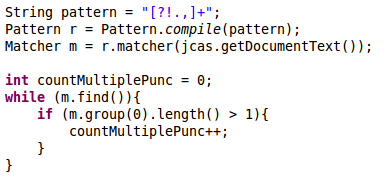
\includegraphics[width=0.6\textwidth]{fig/multiplepunc.png}
    \caption[Short caption]{Piece of code for the multiple punctuation feature}
    \label{fig:multipunc}
\end{figure}
\
This feature can be a good representation of aggressiveness and poor argumentation in a debate, as it can be seen in the following example:
\\
\fbox{\begin{minipage}{1\textwidth}
\textbf{208\_P2\_artcomment\_homeschooling.txt} smarmy bastard 2011/09/19 at 6:00 PM "…ok so obviously , there are more free thinkers who would agree with you, .... and because there are more than one free thinker(s) , it becomes a group of free thinkers ...who all agree ... hmmm (head hits floor)" \_\_\_ 
Smarmy: now you're just being disagreeable. If many people independently think for themselves, without being told what, when, and how to think, it does not follow that they all think the same thing. "Following" is an attribute reserved for religion. 
Me thinks your head may have hit the floor too hard this time.
\end{minipage}}

\subsubsection{Multiple Capital Letters}
Another feature that can reflect the lack of seriousness is the number of words with multiple capital letters. In the following example, there are 3 words with multiple capital letters:
\\
\\
\fbox{\begin{minipage}{1\textwidth}
\textbf{3144\_P2\_artcomment\_public-private-schools.txt} WRONG - NO !! Perhaps bad psychology, bad child rearing, perhaps. They are paying for the public schools, its called  TAXES!! 
\end{minipage}} 	 	

\subsection{Part Of Speech Features}
In grammar, parts of speech (abbreviation: POS) are the linguistic categories of words such as verb, noun, ect... In DKPro the POS are modelled as subclasses of the class \emph{POS}, which is an annotation. 

\subsubsection{Ratio on common POS}
One simple feature, already implemented in DKPro\footnote{In TC Google code, have a look at de/tudarmstadt/ukp/dkpro/tc/features/syntax/POSRatioFeatureExtractor.java}, computes 11 ratios of 11 different over the total number of POS:

\begin{table}[h]
\center
\begin{tabular}{|l|l|l|}
\hline
\rowcolor[HTML]{9B9B9B} 
POS             & Abbreviation & Examples         \\ \hline
Adjective       & ADJ          & good, tall       \\ \hline
Adverb          & ADV          & quickly, lightly \\ \hline
Article         & ART          & a, the           \\ \hline
Cardinal Number & CARD         & one, eighty-two  \\ \hline
Conjunction     & CONJ         & for, and         \\ \hline
Noun            & N            & cat, Germany     \\ \hline
Exclamation     & O            & O, oh!           \\ \hline
Preposition     & PP           & above, within    \\ \hline
Pronoun         & PR           & I, she           \\ \hline
Punctuation     & PUNC         & ``.", ``;"       \\ \hline
Verb            & V            & to be, had       \\ \hline
\end{tabular}
\caption{\label{11pos} The 11 POS we consider for the Ratio POS feature}
\end{table}

??TODO: Investigate why no all the black lines

The DKPro functions allow to compute the ratios and thus create the features very easily as seen on \cref{fig:11poscode}.
\
\begin{figure}[H]
    \centering
    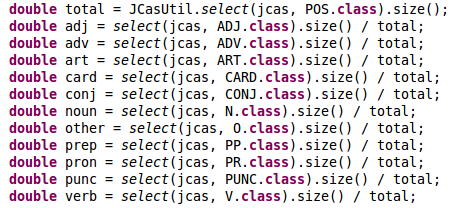
\includegraphics[width=0.6\textwidth]{fig/11pos.png}
    \caption[Short caption]{Piece of code for the multiple punctuation feature}
    \label{fig:11poscode}
\end{figure}
\
\subsubsection{Comparative and Superlative}
The previous features don't consider the ratios of comparative and superlative (for adverbs and adjectives) in a text but they are relevant in debates since opponents usually keep on comparing the different point of views.

\subsubsection{Modal Verbs}
Again, in a more granulate analysis, we can evaluate the ratios for the 9 common ratios in English: can, could, may, might, must, shall, should, will and would.

\subsubsection{POS N-Grams}
By analogy with the Token NGrams feature, DKPro has a POS NGrams feature. As an example, if you consider the sentence:

\begin{table}[h]
\center
\begin{tabular}{cccccc}
This & Virginia & law & is & insane & .    \\
\texttt{ART}  & \texttt{NP}       & \texttt{NN}  & \texttt{V}  & \texttt{ADJ}    & \texttt{PUNC}
\end{tabular}
\end{table}\
\\
The POS 1-grams are: \texttt{ART, NP, NN, V, ADJ, PUNC}
\\
The POS 2-grams are: \texttt{ART\_NP, NP\_NN, NN\_V, V\_ADJ, ADJ\_PUNC}
\\
and so on \ldots
\\
Unfortunately, the POS n-grams tend to introduce some noise and redundancy in our classification, so we won't use them much.

\subsection{Syntactic features}
The \emph{syntax} is the study of how languages are constructed in a certain language. We'll define in this part the syntax related. Syntax is very descriptive, most of the syntactic representations of sentences, texts are often graphs, tables, ect... We'll see how we came with the quantitative features needed to perform the classification.

\subsubsection{Depth of the Dependency Tree}
\textbf{Dependency Tree}
\\
\\
In V {\'A}gel's works \cite{ágel2006dependency}, the dependency tree is a graph that maps the relations between the different grammar units in a sentence. The theory behind is long long and arduous and we leave to the reader the study of dependency trees. Nevertheless, we give in the following figure (\ref{fig:deptree}), a simple example of a dependency tree.

For the sentence \texttt{I shot an elephant in my pajamas}, we get the following tree:
\
\begin{figure}[H]
    \centering
    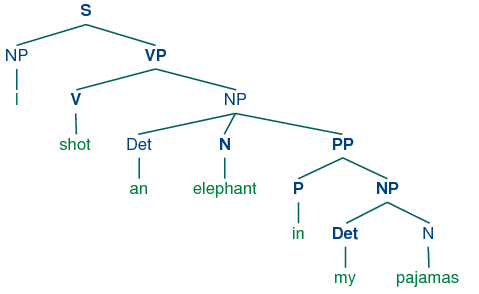
\includegraphics[width=0.7\textwidth]{fig/deptree.png}
    \caption[Short caption]{A dependency tree}
    \label{fig:deptree}
\end{figure}
\
To quantify how complex a sentence can be, we took inspiration on Christian Stab work on Argumentative Discourse \cite{TUD-CS-2014-0882} by calculating the depth of the dependency tree for every sentence. The depth of a tree is the number of edges between the first node and the furthest extremity in the tree. In \cref{fig:deptree}, the depth of the tree is 5.
\
\begin{figure}[H]
    \centering
    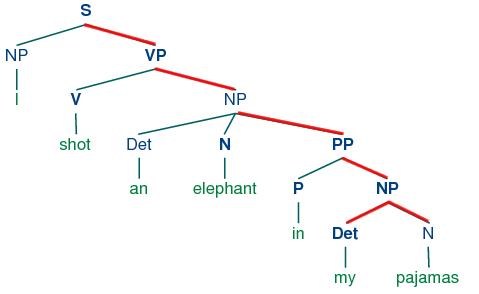
\includegraphics[width=0.7\textwidth]{fig/deptreepath.png}
    \caption[Short caption]{5 edges between the summit S and the extremities Det and N}
    \label{fig:deptreepath}
\end{figure}
\








